\subsection{Resultados do treinamento com o \textit{dataset Mardini} (Espanhol) usando o Modelo \textit{BETO Base}}

Os resultados para o \textit{dataset Mardini} em espanhol utilizando o modelo \textit{BETO Base} demonstram uma acurácia média variando entre 65.12\% e 71.7\%. A acurácia mais alta foi alcançada com 90\% dos dados de treinamento. Os valores de EQM e EMA são relativamente estáveis, com uma leve melhoria à medida que a quantidade de dados de treinamento aumenta. Estes resultados indicam que o modelo \textit{BETO Base} é eficaz para tarefas em espanhol, embora haja espaço para melhorias no uso de outra versão do modelo, como veremos na comparação a versão \textit{Large}.

\begin{table}[h!]
\centering
\resizebox{\columnwidth}{!}{%
\begin{tabular}{|p{0.25\textwidth}|p{0.1\textwidth}|p{0.1\textwidth}|p{0.4\textwidth}|p{0.1\textwidth}|p{0.1\textwidth}|p{0.1\textwidth}|}
    \hline
    \textbf{Percentual de dados para o treinamento} & \textbf{Qtd. Treino} & \textbf{Qtd. Teste} & \textbf{Pesos [Fator 1, Fator 2, Fator 3]} & \textbf{EQM} & \textbf{EMA} & \textbf{Acurácia média} \\
    \hline
     60\% & 2263 & 1509 & [0.0838, 0.0349, 0.4526] & 0.8955 & 0.7457 & 65.12\% \\
    \hline
     70\% & 2640 & 1132 & [0.1119, 0.0387, 0.4619] & 0.9010 & 0.7536 & 66.58\% \\
    \hline
     80\% & 3017 & 755 & [0.1077, 0.0453, 0.4709] & 0.8702 & 0.7390 & 66.28\% \\
    \hline
     90\% & 3394 & 378 & [0.1034, 0.0486, 0.4504] & 0.8822 & 0.7449 & 71.7\% \\
    \hline
\end{tabular}%
}
\caption{Resultados de Regressão para Diferentes Percentuais de Treino com o \textit{dataset Mardini} (Espanhol) usando o Modelo \textit{BETO Base}}
\label{tab:resultados_regressao_espanhol_base}
\end{table}

Nos gŕafico das Figuras \ref{figure:4} é possível ver uma quantidade grande de erros distribuídos em varias faixas, ao passo que na Figura \ref{figure:7} esses erros diminuíram, e a faixa mais concetrada é a de entre 20\% e 30\% de divergência nas avaliações do algoritmo comparadas com as avaliações dos professores.

\begin{figure}[h!]
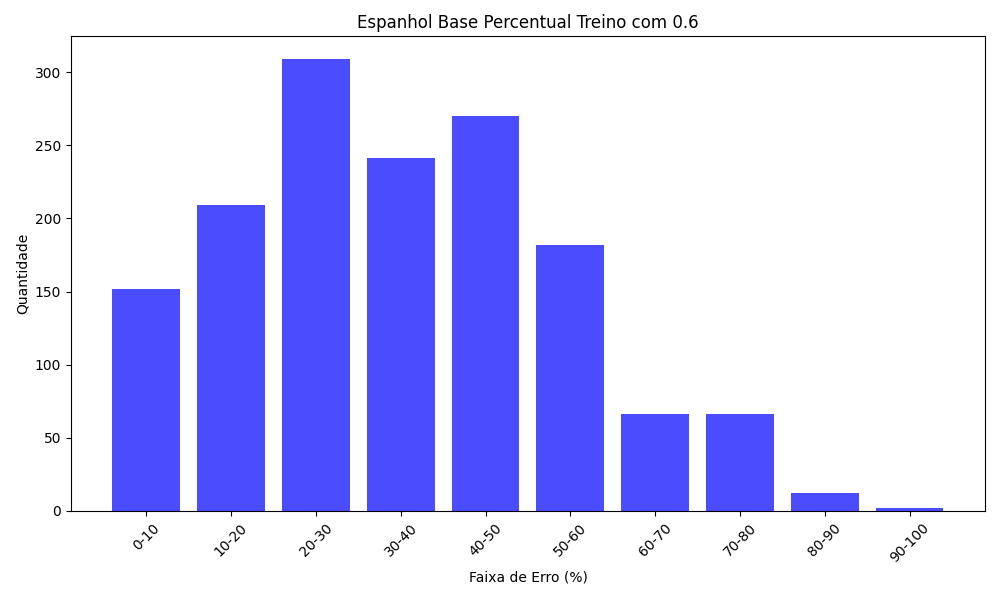
\includegraphics[width=\textwidth]{img/grafsEsp/Espanhol Base Percentual Treino com 0.6_quantidade.png}
\caption{Quantidade de respostas por faixas de erro percentual dos testes com 40\% do \textit{dataset Mardini} (Espanhol) usando o Modelo \textit{BETO Base}}\label{figure:4}
\end{figure}

\begin{figure}[h!]
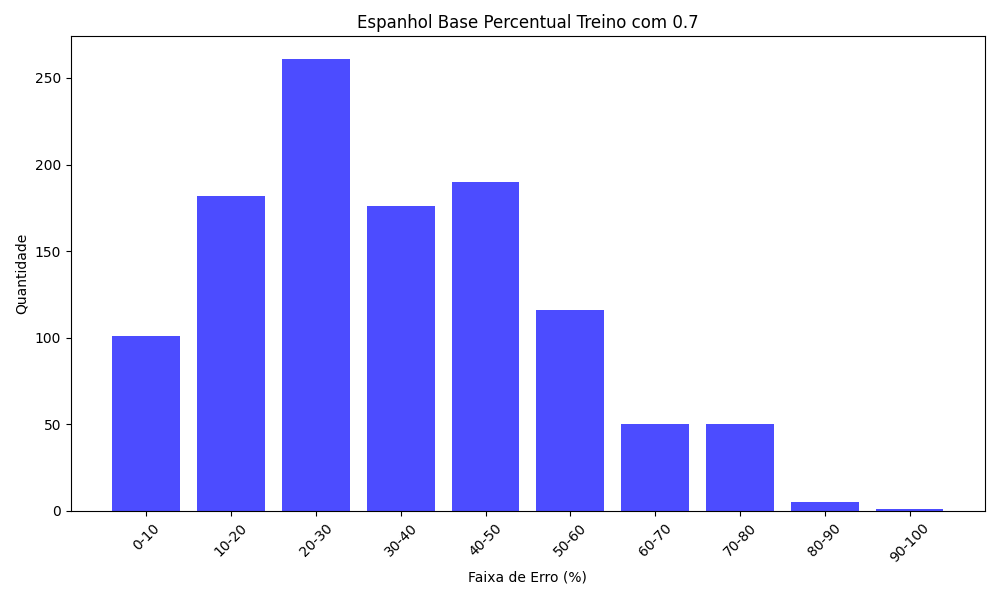
\includegraphics[width=\textwidth]{img/grafsEsp/Espanhol Base Percentual Treino com 0.7_quantidade.png}
\caption{Quantidade de respostas por faixas de erro percentual dos testes com 30\% do \textit{dataset Mardini} (Espanhol) usando o Modelo \textit{BETO Base}}\label{figure:5}
\end{figure}

\begin{figure}[h!]
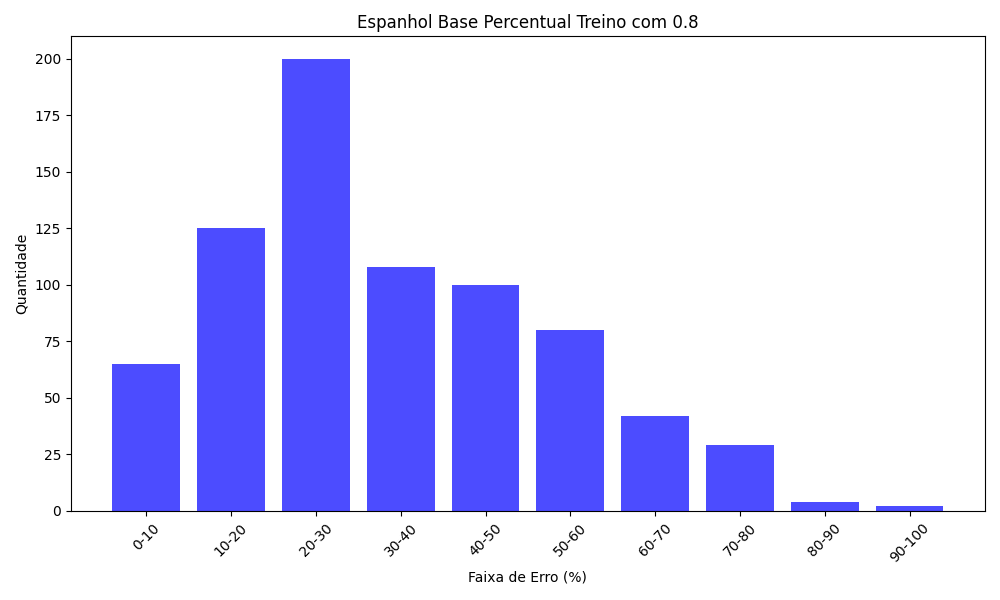
\includegraphics[width=\textwidth]{img/grafsEsp/Espanhol Base Percentual Treino com 0.8_quantidade.png}
\caption{Quantidade de respostas por faixas de erro percentual dos testes com 20\% do \textit{dataset Mardini} (Espanhol) usando o Modelo \textit{BETO Base}}\label{figure:6}
\end{figure}

\begin{figure}[h!]
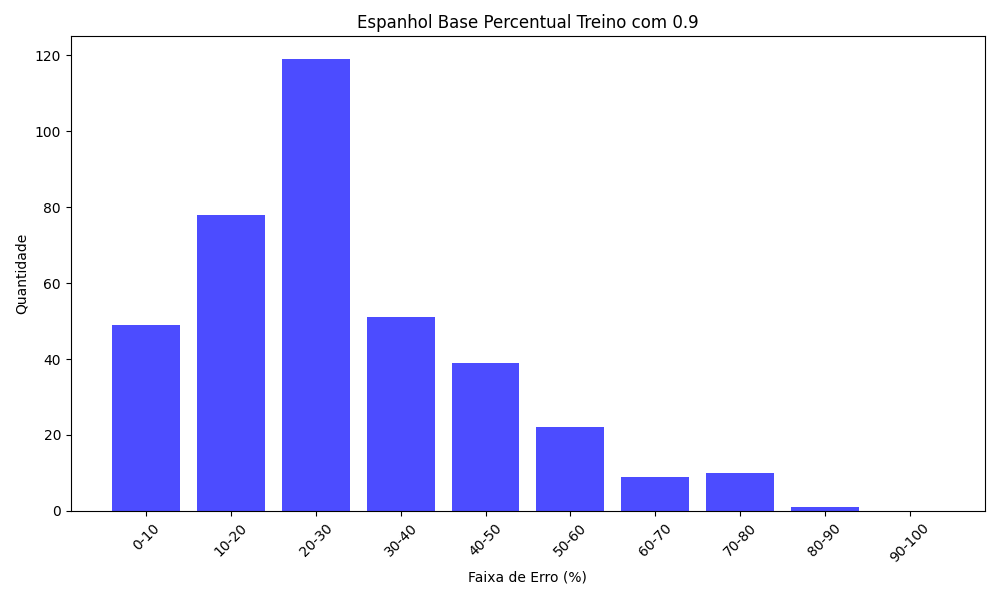
\includegraphics[width=\textwidth]{img/grafsEsp/Espanhol Base Percentual Treino com 0.9_quantidade.png}
\caption{Quantidade de respostas por faixas de erro percentual dos testes com 10\% do \textit{dataset Mardini} (Espanhol) usando o Modelo \textit{BETO Base}}\label{figure:7}
\end{figure}

\FloatBarrier

%-------------------------------------------

\subsection{Resultados do treinamento com o \textit{dataset Mardini} (Espanhol) usando o Modelo \textit{BETO Large}}

Para o \textit{dataset Mardini} em espanhol utilizando o modelo \textit{BETO Large}, os resultados mostram uma acurácia média superior, variando de 78.14\% a 83.58\%. A acurácia mais alta foi obtida com 90\% dos dados de treinamento. Os valores de EQM e EMA são ligeiramente melhores comparados ao modelo \textit{BETO Base}, confirmando que o \textit{BETO Large} oferece um desempenho aprimorado em tarefas de processamento de linguagem natural em espanhol.

\begin{table}[h!]
\centering
\resizebox{\columnwidth}{!}{%
\begin{tabular}{|p{0.25\textwidth}|p{0.1\textwidth}|p{0.1\textwidth}|p{0.4\textwidth}|p{0.1\textwidth}|p{0.1\textwidth}|p{0.1\textwidth}|}
    \hline
    \textbf{Percentual de dados para o treinamento} & \textbf{Qtd. Treino} & \textbf{Qtd. Teste} & \textbf{Pesos [Fator 1, Fator 2, Fator 3]} & \textbf{EQM} & \textbf{EMA} & \textbf{Acurácia média} \\
    \hline
    60\% & 2263 & 1509 & [0.1412, 0.0081, 0.1289] & 0.9622 & 0.7773 & 78.14\% \\
    \hline
    70\% & 2640 & 1132 & [0.1634, 0.0049, 0.1366] & 0.9703 & 0.7835 & 78.74\% \\
    \hline
    80\% & 3017 & 755 & [0.1638, 0.0010, 0.1300] & 0.9450 & 0.7754 & 79.18\% \\
    \hline
    90\% & 3394 & 378 & [0.1509, 0.0085, 0.1439] & 0.9441 & 0.7783 & 83.58\% \\
    \hline
\end{tabular}%
}
\caption{Resultados de Regressão para Diferentes Percentuais de Treino com o \textit{dataset Mardini} (Espanhol) usando o Modelo \textit{BETO Large}}
\label{tab:resultados_regressao_espanhol_large}
\end{table}

Nos gŕafico das Figuras \ref{figure:8}, \ref{figure:9}, \ref{figure:10} e \ref{figure:11} é possível ver que a maiora das avaliações se mantém na faixa de acurácia acima de 70\%, com uma mudança na distribuiçao comparando com o modelo \textit{Base}.

\begin{figure}[h!]
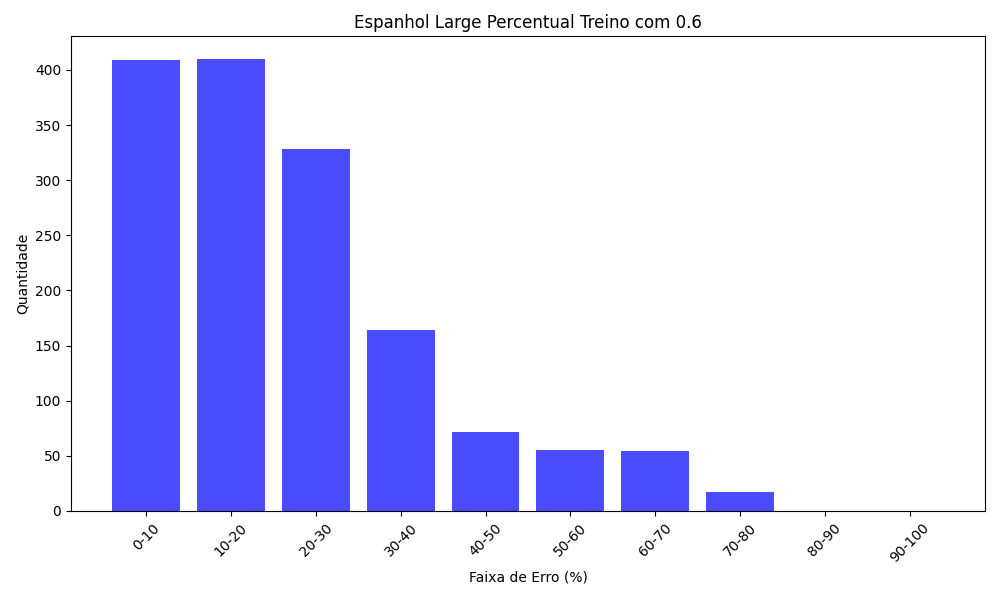
\includegraphics[width=\textwidth]{img/grafsEsp/Espanhol Large Percentual Treino com 0.6_quantidade.png}
\caption{Quantidade de respostas por faixas de erro percentual dos testes com 40\% do \textit{dataset Mardini} (Espanhol) usando o Modelo \textit{BETO Large}}\label{figure:8}
\end{figure}

\begin{figure}[h!]
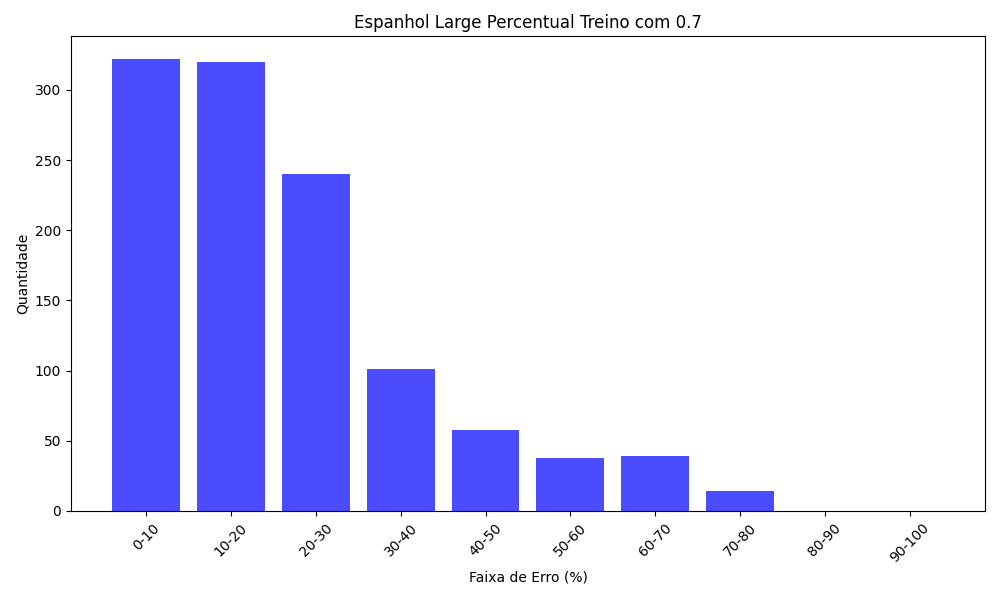
\includegraphics[width=\textwidth]{img/grafsEsp/Espanhol Large Percentual Treino com 0.7_quantidade.png}
\caption{Quantidade de respostas por faixas de erro percentual dos testes com 30\% do \textit{dataset Mardini} (Espanhol) usando o Modelo \textit{BETO Large}}\label{figure:9}
\end{figure}

\begin{figure}[h!]
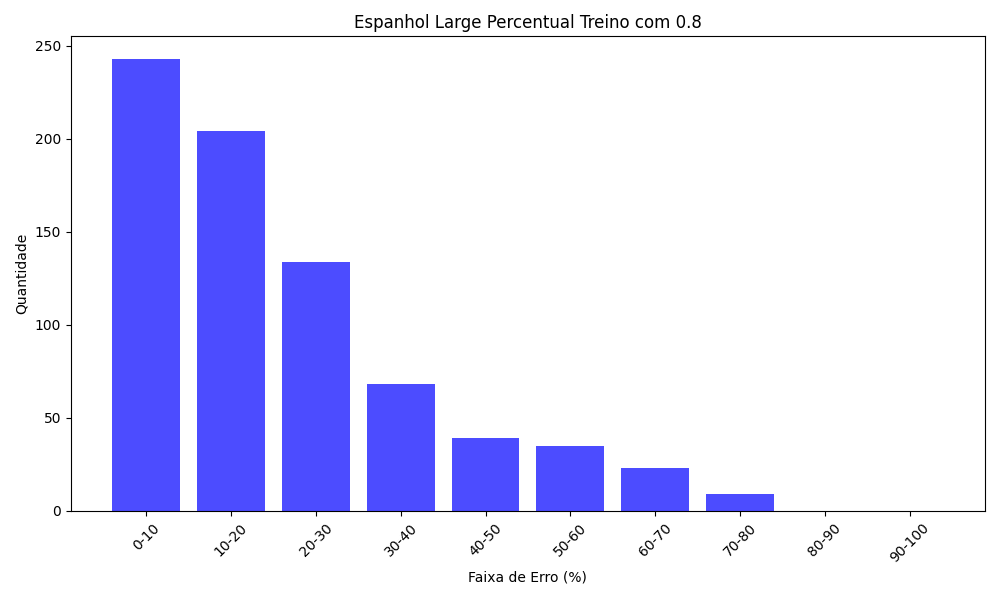
\includegraphics[width=\textwidth]{img/grafsEsp/Espanhol Large Percentual Treino com 0.8_quantidade.png}
\caption{Quantidade de respostas por faixas de erro percentual dos testes com 20\% do \textit{dataset Mardini} (Espanhol) usando o Modelo \textit{BETO Large}}\label{figure:10}
\end{figure}

\begin{figure}[h!]
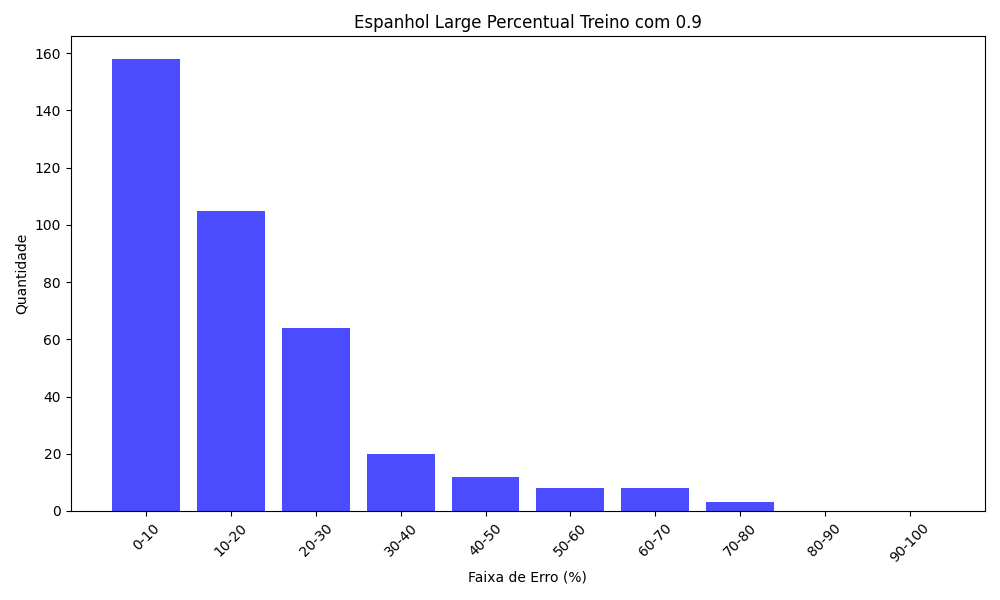
\includegraphics[width=\textwidth]{img/grafsEsp/Espanhol Large Percentual Treino com 0.9_quantidade.png}
\caption{Quantidade de respostas por faixas de erro percentual dos testes com 10\% do \textit{dataset Mardini} (Espanhol) usando o Modelo \textit{BETO Large}}\label{figure:11}
\end{figure}

\FloatBarrier

%-------------------------------------------

% \subsection{Resultados do treinamento com o \textit{dataset} Espanhol usando o Modelo ROBERTA (Quantidade de dados: 3772)}

% \begin{table}[h!]
% \centering
% \resizebox{\columnwidth}{!}{%
% \begin{tabular}{|p{0.25\textwidth}|p{0.1\textwidth}|p{0.1\textwidth}|p{0.4\textwidth}|p{0.1\textwidth}|p{0.1\textwidth}|p{0.1\textwidth}|}
%     \hline
%     \textbf{Percentual de dados para o treinamento} & \textbf{Qtd. Treino} & \textbf{Qtd. Teste} & \textbf{Pesos [Fator 1, Fator 2, Fator 3]} & \textbf{EQM} & \textbf{EMA} & \textbf{Acurácia média} \\
%     \hline
%     60\% & 2263 & 1509 & [0.1782, 0.0090, 0.1067] & 0.9754 & 0.7780 & 74.5\% \\
%     \hline
%     70\% & 2640 & 1132 & [0.2071, 0.0208, 0.1106] & 0.9852 & 0.7867 & 74.98\% \\
%     \hline
%     80\% & 3017 & 755 & [0.2039, 0.0283, 0.1627] & 0.9508 & 0.7734 & 72.66\% \\
%     \hline
%     90\% & 3394 & 378 & [0.1949, 0.0387, 0.1686] & 0.9526 & 0.7774 & 76.27\% \\
%     \hline
% \end{tabular}%
% }
% \caption{Resultados de Regressão para Diferentes Percentuais de Treino com o \textit{dataset} Espanhol usando o modelo ROBERTA}
% \label{tab:resultados_regressao_roberta_espanhol}
% \end{table}

% \begin{figure}[h!]
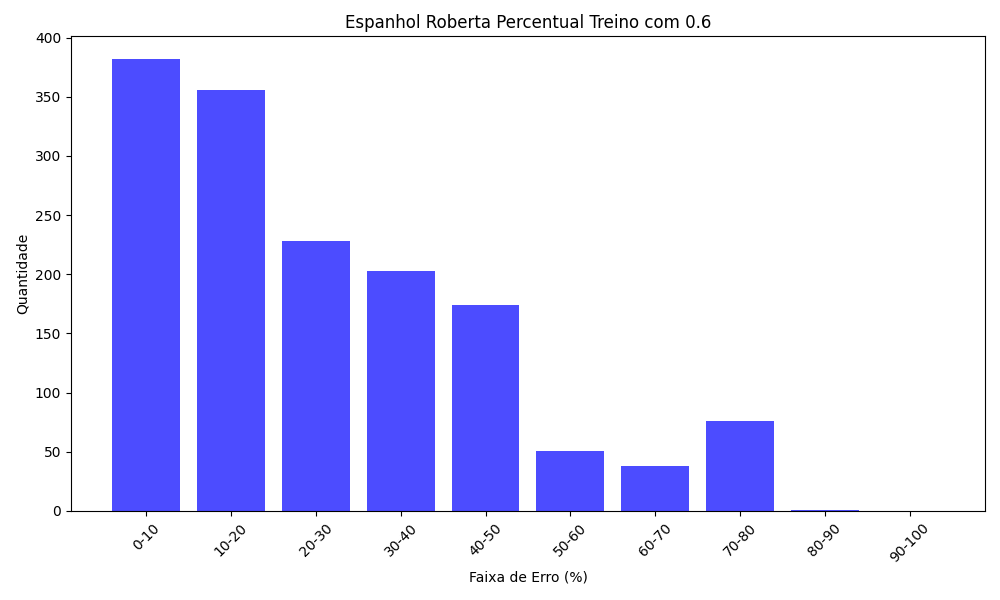
\includegraphics[width=\textwidth]{img/grafsEsp/Espanhol Roberta Percentual Treino com 0.6_quantidade.png}
\caption{Quantidade de respostas por faixas de erro percentual dos testes com 40\% do \textit{dataset} (Modelo Espanhol \textit{ROBERTA})}\label{figure:12}
\end{figure}

\begin{figure}[h!]
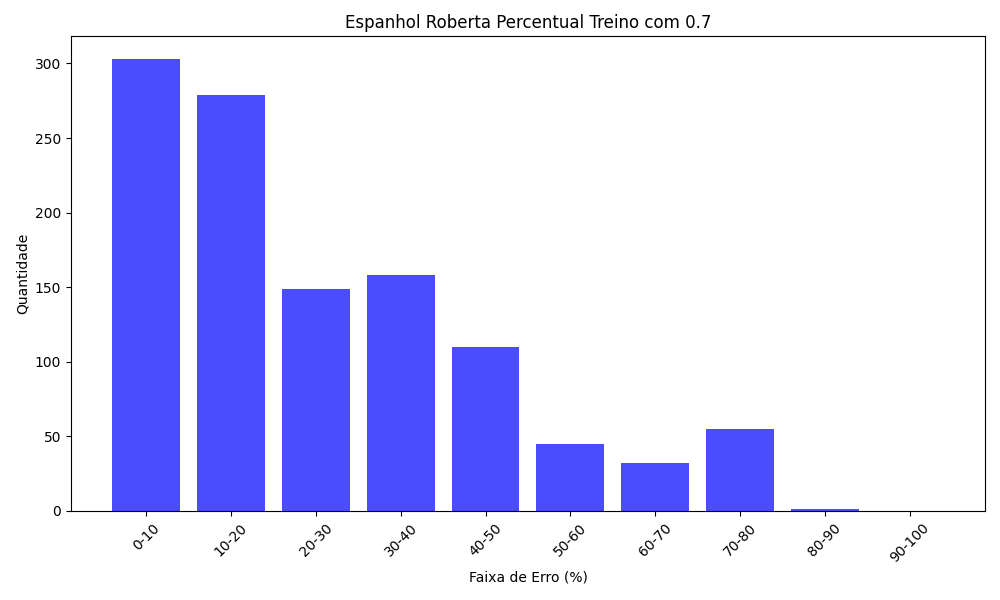
\includegraphics[width=\textwidth]{img/grafsEsp/Espanhol Roberta Percentual Treino com 0.7_quantidade.png}
\caption{Quantidade de respostas por faixas de erro percentual dos testes com 30\% do \textit{dataset} (Modelo Espanhol \textit{ROBERTA})}\label{figure:13}
\end{figure}

\begin{figure}[h!]
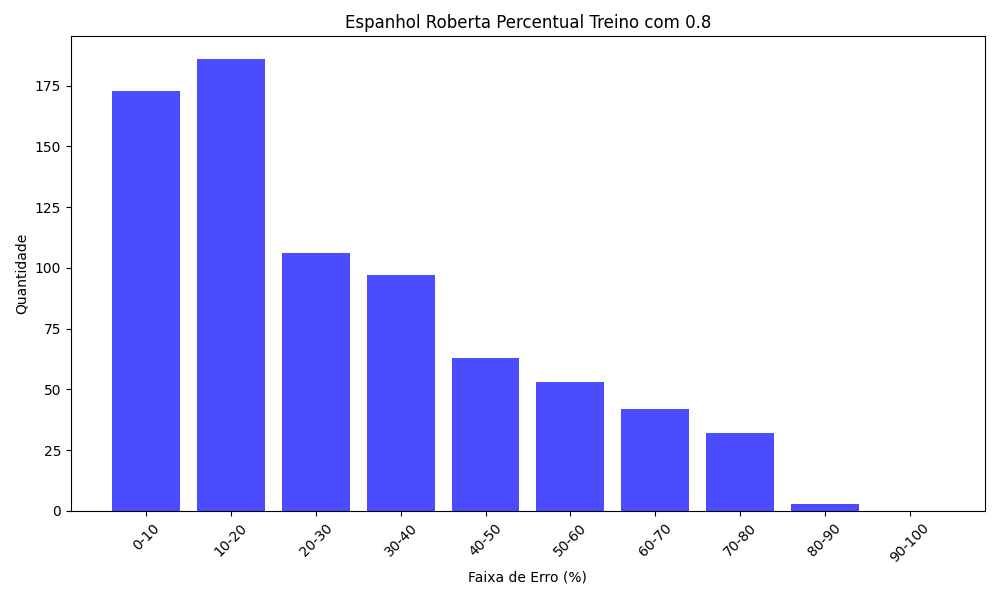
\includegraphics[width=\textwidth]{img/grafsEsp/Espanhol Roberta Percentual Treino com 0.8_quantidade.png}
\caption{Quantidade de respostas por faixas de erro percentual dos testes com 20\% do \textit{dataset} (Modelo Espanhol \textit{ROBERTA})}\label{figure:14}
\end{figure}

\begin{figure}[h!]
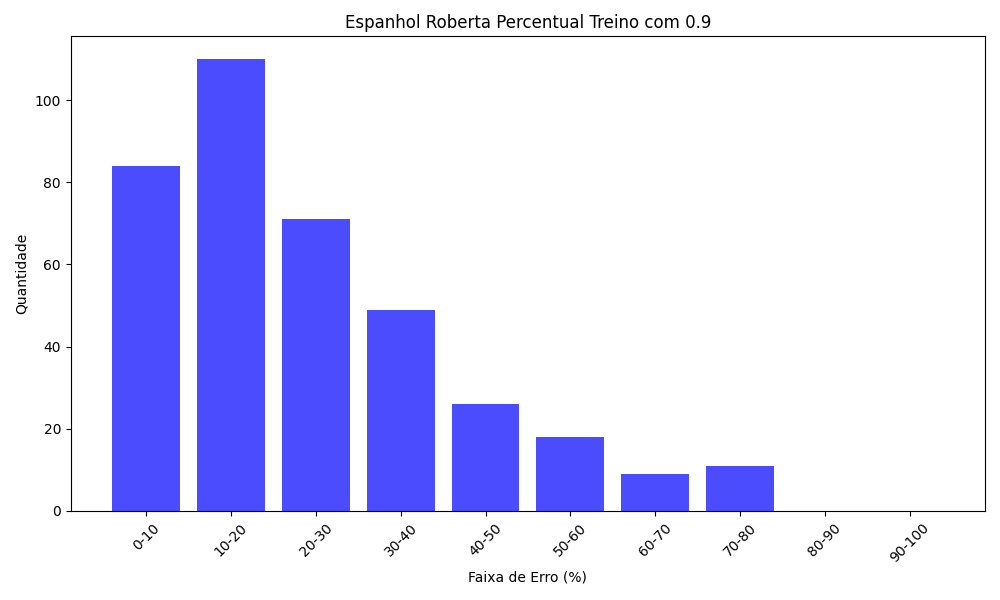
\includegraphics[width=\textwidth]{img/grafsEsp/Espanhol Roberta Percentual Treino com 0.9_quantidade.png}
\caption{Quantidade de respostas por faixas de erro percentual dos testes com 10\% do \textit{dataset} (Modelo Espanhol \textit{ROBERTA})}\label{figure:15}
\end{figure}

% \FloatBarrier